\documentclass{beamer}

\def\Tiny{\fontsize{6pt}{6pt}\selectfont}
\def\supertiny{\fontsize{4pt}{4pt}\selectfont}

\mode<presentation>
{
  \usetheme{Warsaw}
  % \setbeamercovered{transparent}
  \usecolortheme{crane}
}

\usepackage{graphicx, ifthen, listings, fancyvrb}

\usepackage[czech]{babel}
% \usefonttheme{professionalfonts}
\usepackage{times}
\usepackage{amsmath}
\usepackage[utf8]{inputenc}
\usepackage{wrapfig}

\usepackage[T1]{fontenc}

\lstset{ basicstyle=\tiny, stringstyle=\ttfamily, showstringspaces=false }

\everymath{\displaystyle}

\setbeamerfont{frametitle}{size=\large}
\setbeamerfont{subsection in toc}{size=\scriptsize}

\makeatletter\newenvironment{blackbox}{%
   \begin{lrbox}{\@tempboxa}\begin{minipage}{0.95\columnwidth}}{\end{minipage}\end{lrbox}%
   \colorbox{black}{\usebox{\@tempboxa}}
}\makeatother

\title[IMF (11)]{Informatika pro moderní fyziky (11)\\ web scraping; API; zadání zápočtových úloh}

\author[Franti\v{s}ek HAVL\r{U}J, ORF ÚJV Řež]{Franti\v{s}ek HAVL\r{U}J\\{\scriptsize \emph{e-mail: haf@ujv.cz}}}

\date{akademický rok 2014/2015\\10. prosince 2014}

\institute[ORF ÚJV Řež]
{ÚJV Řež\\oddělení Reaktorové fyziky a podpory palivového cyklu}

\AtBeginSection[]
{
\begin{frame}<beamer>
\frametitle{Obsah}
\tableofcontents[currentsection,hideothersubsections]
\end{frame}
}

\begin{document}

\begin{frame}
  \titlepage
\end{frame}

\begin{frame}
  \tableofcontents
\end{frame}

\section{K zápočtovým úlohám}

\begin{frame}{Obecně:}
\begin{itemize}
  \item ke každému zadání jsou k dispozici vzorová data
  \item já to budu testovat i na datech jiných
  \item očekávám, že všechno proběhne na jedno spuštění skriptu / rake tasku
  \item každý má k dispozici jeden pokus řádný a jeden opravný
\end{itemize}
\end{frame}

\begin{frame}{Klasifikace}
  \begin{itemize}
    \item F - nejde to spustit, ani pro zadaná data to v podstatných bodech nesplňuje zadání
    \item E - pro zadaná data to funguje, ale pro jiná čísla to nechodí
    \item D - obecně to funguje, ale stejně chybí drobnosti ze zadání
    \item C - všechno funguje jak má
    \item B - funguje a navíc jsou výstupy hezké a přehledné, soubory nejsou generovány “na velkou hromadu”, ale roztříděné do složek apod.
    \item A - kromě výše uvedeného jsou splněny i požadavky formy (správné odsazování, rozumná jména funkcí a proměnných) a efektivity (je to rozumně naprogramované - vhodné použití funkcí, datových struktur atd.)
  \end{itemize}
\end{frame}

\begin{frame}{Známka se snižuje o stupeň, pokud:}
  \begin{itemize}
    \item jsou někde ve skriptech použity absolutní cesty, takže je budu muset upravovat (výjimkou jsou cesty k programům jako např. gnuplot, které ovšem musí být umístěny v proměnné někde na začátku skriptu (abych to nemusel lovit)
    \item bude v kódu něco, co limituje použití na OS Windows (backslash v cestě, kódování win1250 atd.)
  \end{itemize}
  (a podobně)
\end{frame}

\begin{frame}{Gamma scanning palivových souborů}
  V souborech assembly*.csv jsou uloženy profily z gamma scanů.
  na prvním řádku je identifikátor kazety
  jednotlivé hodnoty jsou odděleny libovolným počtem mezer nebo novým řádkem -- jedná se o integrální hodnoty signálu z jednotlivých nódů (tedy intenzita * výška nódu)

  Axiální nodalizace je následující: 10 nódů po 1 cm, 8 nódů po 5 cm, 16 nódů po 2 cm, 8 nódů po 5 cm, 10 nódů po 1 cm

  Úkol:
  \begin{itemize}
    \item vykreslit axiální profily intenzity signálů pro všechny PS (podle vzoru)
    \item do jednoho grafu vykreslit profily pěti PS s největší celkovou aktivitou
  \end{itemize}

\end{frame}

\begin{frame}{}
  \begin{center}
    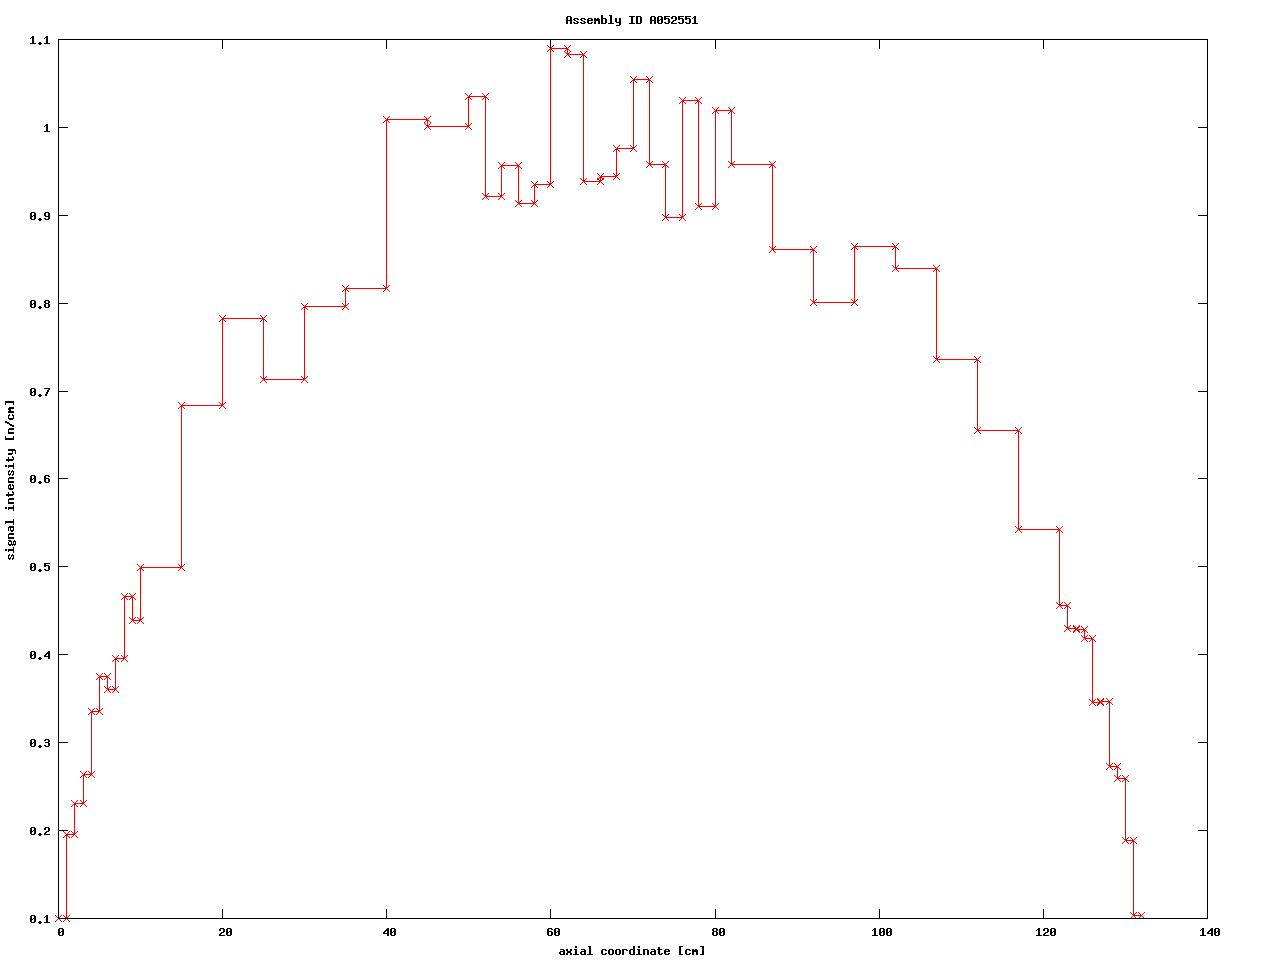
\includegraphics[width=0.8\textwidth]{assembly_001}    
  \end{center}
\end{frame}

\begin{frame}{Databáze vzorků v laboratoři (a,b)}
  Záznamy o vstupu a výstupu vzorků ze skladu - systém zapisuje datum průchodu, ID vzorku a naměřený dávkový příkon (miliSv/den); pro každý vzorek jsou v souboru právě dva záznamy. Pokles dávkového příkonu předpokládejte exponenciální (A * e \^ (-Bx)).

  Úkol:
  
  \begin{itemize}
\item najít vzorek s celkovou nejvyšší a nejnižší dávkou  
\item vykreslit histogram rozložení celkových dávek
\item vykreslete histogram délky pobytu vzorku v laboratoři
\item vykreslete oblak (scatter plot) zobrazující vztah mezi délkou pobytu (osa x) a celkovou aktivitou (osa y)  
  \end{itemize}
\end{frame}

\begin{frame}{Komiks!}
  Komiks XKCD http://xkcd.com
  
  \begin{itemize}
    \item vygenerovat hezké PDF s obsahem (obsahujícím názvy jednotlivých dílů); každý díl včetně popisku (img/alt nebo img/title atribut)
    \item navíc HTML dokument umožňující prohlížení na jedné stránce (bez scrollování) - tedy rozumně vymyšlený seznam v levém sloupci (rozklikávací po částech, aby se nemuselo scrollovat), tlačítko dopředu+zpět
  \end{itemize}

\end{frame}

\begin{frame}[containsverbatim]{Univerzální vykreslovač}
  V adresáři "data" se nachází blíže neurčený počet CSV souborů se záznamem časového průběhu signálů z detektorů. V prvním řádku je záhlaví popisující jednotlivé sloupce, tedy například takto:

\begin{verbatim}
  #y4 y1 y2 y3 time
  1.1059 0.2212 0.1896 0.6777 0.01
  0.2399 0.4539 0.428 1.1479 0.02
\end{verbatim}  

  Sloupec "time" je přítomen právě jeden (nicméně pokaždé na jiné pozici). 

  Každý CSV soubor vykreslete do grafu, na ose X je čas, na ose Y jednotlivé signály -- co soubor to graf, všechny signály z jednoho souboru vykreslené najednou. V legendě názvy sloupců.
  
\end{frame}

\begin{frame}[containsverbatim]{Kartogramy pro VVER-1000}
    Na základě textového kartogramu jedné šestiny aktivní zóny VVER-1000 (levá dolní šestina + centrální PS) vykreslete kartogram celé zóny s barvičkami podle typu palivového souboru. Co dodat.

  Příklad:
  \tiny
\begin{verbatim}
    *     *   A30E9  A20   A13    A20   A30E9   A13    A30E9
       *  A40E6    A20        A13   A30E9   A13    A20
           *   P40E9   A30E9     A13    A20   A13
                *   P36E9   A20      A13   A30E9
                     *   P36E9   A30E9   A13
                           *  P40E9   A20
                                *  A40E6
                                    *  
\end{verbatim}
\end{frame}

\begin{frame}{}
  \begin{center}
    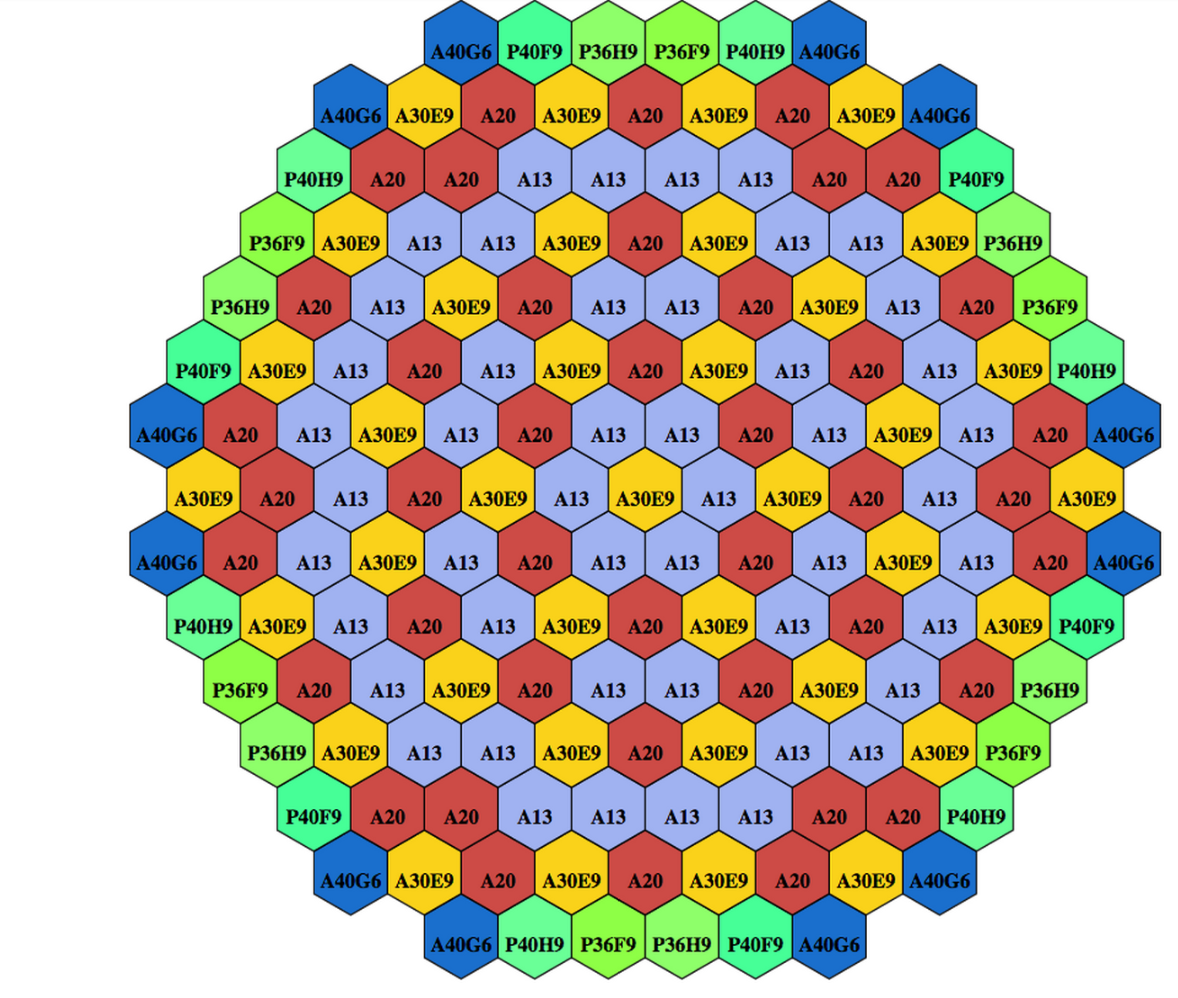
\includegraphics[width=0.6\textwidth]{kartogram}    
  \end{center}
\end{frame}

\section{Navážeme na předminulou hodinu}

\begin{frame}{HTML scraping}
  \begin{itemize}
    \item získávání informací z webu, které nám někdo nechce dát
    \item umíme číst HTML (knihovna \texttt{nokogiri}, případně \texttt{ox}), umíme stahovat soubory, takže dobrý
    \item pozor, občas se hodně informací nahrává až zpožděně přes Ajax a člověk musí použít tzv. \emph{headless browser}, např \texttt{capybara} (ze zkušenosti: sázkové weby) 
  \end{itemize}
\end{frame}

\begin{frame}{Připomenutí obecného postupu}
  \begin{itemize}
    \item najdu URL, které mě zajímá
    \item na stránce hledám vhodný CSS selektor, abych se dostal k tomu, co potřebuju
    \item stáhnu data, která mě zajímají
  \end{itemize}
\end{frame}

\begin{frame}{Nalezení vhodného selektoru}
  \begin{itemize}
    \item v principu hledám minimální formu -- aby tomu vyhovovalo to, co potřebuju, ale nic jiného
    \item pomůžou mi vývojářské nástroje v prohlížeči
    \item obvykle to jde hodně snadno, hlavně pomocí \texttt{class} atributů -- \texttt{element.css("div.comicsImage")} nebo tak něco
    \item klidně to můžu ``dofiltrovat'' až ve skriptu, selektor nemusí být bezchybný 
  \end{itemize}
\end{frame}

\begin{frame}[fragile]{Práce s XML / HTML}
  Knihovna \texttt{nokogiri}
  \scriptsize
\begin{verbatim}
  doc = Nokogiri::HTML(File.open("redmeat.html"))
  doc.css("li.archiveImage a").each do |x|
    url = x.attributes['href']
    ...
  end
\end{verbatim}
\end{frame}

\begin{frame}[fragile]{Knihovna open-uri}
umožňuje otevírat URL jako soubory
  \scriptsize
\begin{verbatim}
require 'open-uri'
doc = Nokogiri::HTML(File.open("http://redmeat.com"))
\end{verbatim}
\end{frame}

\begin{frame}[fragile]{Stahování dat}
  Součást standardní knihovny -- \texttt{open-uri}
  \scriptsize
\begin{verbatim}
  require 'open-uri'
  File.open(local_filename, 'wb') do |f2|
    open(remote_url, 'rb') do |f1|
      f2.write f1.read
    end
  end
\end{verbatim}
\end{frame}


\begin{frame}{Komiks -- TWP}
  \begin{itemize}
    \item \texttt{http://threewordphrase.com/}
    \item otevřu si archiv, tam snadno najdu seznam stránek
    \item na každé stránce je snadné najít ten obrázek (teda ne úplně, ale skoro)
    \item rovnou můžu stáhnout i popisek (atribut \texttt{title}) 
  \end{itemize}
\end{frame}


\section{Použití cizích API}

\begin{frame}{K čemu to?}
  \begin{itemize}
    \item spousta informací na webu je poskytována ve strojově čitelné formě
    \item API -- rozhraní mezi aplikacemi 
    \item s využitím webových služeb naše možnosti exponenciálně rostou
    \item spousta věcí se dá udělat jako \emph{mashup} -- sice nic neumím, ale umím to dát dohromady
  \end{itemize}
\end{frame}


\begin{frame}{Typy / formáty}
  \begin{itemize}
    \item URL -- rovnou dostanu např. obrázek po zadání správného URL
    \item XML -- velmi obecný, ale komplikovaný formát (\"vypadá jako HTML\")
    \item JSON -- velmi jednoduchý a kompaktní formát, vyvinutý pro JS (v podstatě jen číslo, řetězec, pole, hash)
  \end{itemize}
\end{frame}


\begin{frame}{URL API -- google maps}
  \begin{itemize}
    \item stačí správně vymyslet 
    \item pozor na usage limits (v produkci je nutné lokální cache...) 
    \item QR platba: \texttt{http://qr-platba.cz/pro-vyvojare/restful-api/\#generator-image}
    \item Google Maps static API: \texttt{https://developers.google.com/maps/documentation/staticmaps/}
  \end{itemize}
\end{frame}


\begin{frame}{JSON API -- počasí}
  \begin{itemize}
    \item \texttt{http://openweathermap.org/}
    \item aktuální počasí -- \texttt{http://api.openweathermap.org/data/2.5/weather?q=Prague}
    \item úkol: vypište předpovězená minima a maxima teploty v následujících deseti dnech ve svém rodném městě
    \item \texttt{http://api.openweathermap.org/data/2.5/forecast/daily?q=Prague\&cnt=10\&mode=json} ...
  \end{itemize}
\end{frame}

\begin{frame}{Práce s JSON}
  \begin{itemize}
    \item v Ruby je k mání knihovna -- \texttt{require `json'}
    \item generování JSON: \texttt{hash.to\_json}
    \item čtení JSON: \texttt{JSON[data]}
    \item hodí se i na serializaci (uložit si hash do souboru) 
  \end{itemize}
\end{frame}


\begin{frame}{XML API -- kalendář o-závodů}
  \begin{itemize}
    \item ORIS API -- http://oris.orientacnisporty.cz/API
    \item úkol: vypišme kalendář MTBO závodů v roce 2015
    \item \texttt{http://oris.orientacnisporty.cz/API/?format=xml\&method=getEventList\&sport=3} ...
  \end{itemize}
\end{frame}



\begin{frame}{A to je vše, přátelé!}
  \begin{center}
    
\includegraphics[width=0.8\textwidth]{looney_tunes}
  \end{center}
\end{frame}

\end{document}
